\newpage
\phantomsection
\chapter{Estudio financiero}

    Este capítulo determina la viabilidad económica y financiera de KERALYTIX. Las primeras secciones resumen el estudio de mercado, la factibilidad, el presupuesto y la gestión de riesgos, que sirven de contexto. La sección Viabilidad económica y financiera define luego cómo se financia el proyecto y calcula el precio final, la TREMA, el VAN y la TIR, siguiendo los criterios de la Guía de costos y evaluación de factibilidad del proyecto~\cite{guia_costos}.

\section{Estudio de mercado}

    \phantomsection
    \subsection{Usuarios y usos}

        Sus usuarios de KERALYTIX son los oftalmólogos generales, los especialistas en córnea y los técnicos de centros de optometría de alta complejidad de Misiones que cuentan con equipos de topografía o tomografía corneal.

        \begin{figure}[H]
            \centering
            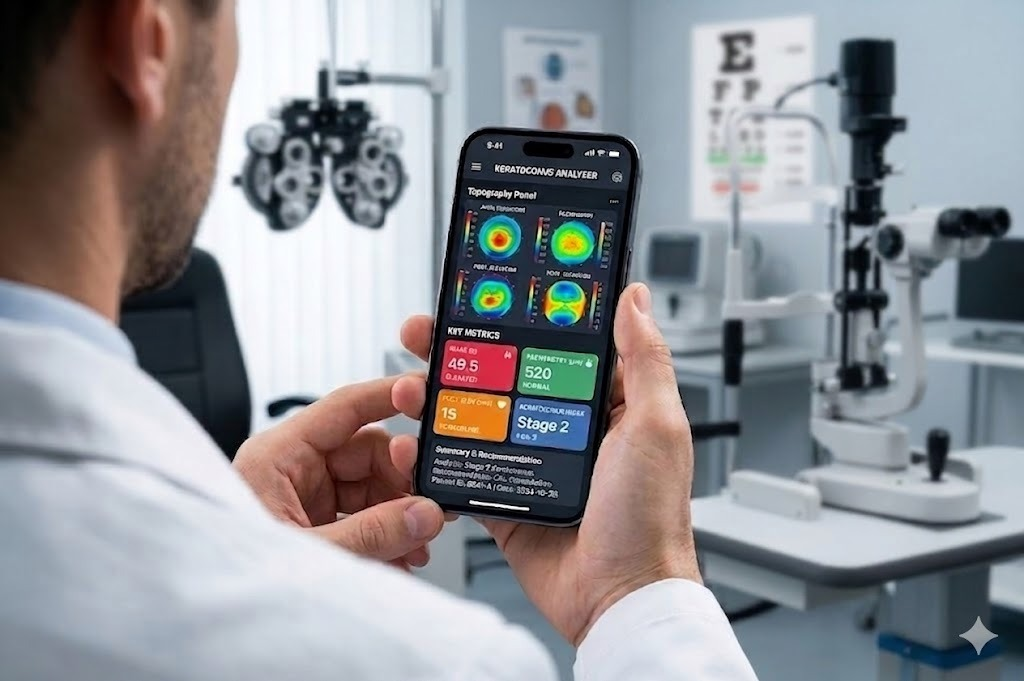
\includegraphics[width=0.5\linewidth]{img/humo.jpeg}
            \caption{Representación visual de la aplicación.}
        \end{figure}

    \phantomsection
    \subsection{Análisis de demanda}

        Existe una necesidad creciente de una herramienta de este tipo derivada de la naturaleza subjetiva del análisis de los estudios. La Tabla~\ref{tabla:demanda} resume los factores que la sustentan.

        \begingroup \setstretch{1.1}
        \vspace{0.3cm}\noindent\begin{talltblr}[
            caption = Factores que sustentan la demanda de KERALYTIX,
            label = tabla:demanda
            ]{
                colspec = {Q[l,m,3.4cm] X[l,m] Q[c,m,2.4cm]},
                cells = {font=\small},
                row{1} = {bg=gray!15, font=\small\bfseries, halign=c},
                hlines, vlines,
                rowsep = 3pt, colsep = 5pt
            }

            Factor & Sustento & Fuente \\

            Subjetividad diagnóstica & La interpretación depende de la experiencia del oftalmólogo, lo que aumenta los errores en etapas subclínicas, que se confunden con enfermedades más comunes. & \cite{deteccion_temprana} \\

            Volumen local de casos & Aumento reportado de casos de queratocono en Oberá, que requieren un diagnóstico preciso. & \cite{misiones} \\

            Descentralización de la atención & Una primera evaluación asistida permite derivar a los centros de alta complejidad solo los casos que lo requieren. & Análisis del problema \\

            Marco normativo & Disposiciones de la ANMAT que encuadran el \textit{software} como producto médico y respaldan la modernización tecnológica en salud. & \cite{dispo_2318,dispo_9688} \\

        \end{talltblr}\par\vspace{0.3cm}
        \endgroup

    \phantomsection
    \subsection{Análisis de la oferta}

        El mercado está dominado por un grupo reducido de fabricantes que venden sistemas cerrados, cuyo \textit{software} de análisis solo funciona con sus propios equipos y no emite una predicción diagnóstica. En el país no existen competidores directos con un \textit{software} como producto médico específico para queratocono. Los aportes y las limitaciones de cada alternativa se resumen en la Tabla~\ref{tabla_antecedentes_comparativa} del capítulo Contextualización.

    \phantomsection
    \subsection{Análisis de precios}

        La Tabla~\ref{tabla:precios_competencia} compara la forma de cobro de la competencia con la de KERALYTIX, y la Tabla~\ref{tabla:estructura_costos} resume la estructura de costos sobre la que se define el precio final (ver sección Viabilidad económica y financiera).

        \begingroup \setstretch{1.1}
        \vspace{0.3cm}\noindent\begin{talltblr}[
            caption = Comparativa de precios de la oferta competitiva,
            label = tabla:precios_competencia
            ]{
                colspec = {Q[l,m,3.8cm] X[l,m] X[l,m]},
                cells = {font=\small},
                row{1} = {bg=gray!15, font=\small\bfseries, halign=c},
                hlines, vlines,
                rowsep = 3pt, colsep = 5pt
            }

            Competidor & Inversión inicial & Modelo de facturación \\

            Sistemas tradicionales (OCULUS / Ziemer) & USD 20.000 a USD 40.000 por equipo, con el \textit{software} incluido & Licencia cerrada, ligada al equipo \\

            Referente local de IA (Entelai) & No requiere \textit{hardware} propio & Pago por informe: $\approx$\,\$\,3.790 + IVA~\cite{entelai} \\

            \textbf{KERALYTIX} & No requiere \textit{hardware} nuevo: procesa los mapas que exportan los equipos existentes & Suscripción mensual de \$\,180.000 por centro \\

        \end{talltblr}\par\vspace{0.3cm}
        \endgroup

        \vspace{-0.5 cm}
        \begingroup \setstretch{1.1}
        \vspace{0.3cm}\noindent\begin{talltblr}[
            caption = Estructura de costos de KERALYTIX,
            label = tabla:estructura_costos
            ]{
                colspec = {X[l,m] Q[c,m,3.2cm] Q[r,m,3.4cm]},
                cells = {font=\small},
                row{1} = {bg=gray!15, font=\small\bfseries, halign=c},
                hlines, vlines,
                rowsep = 3pt, colsep = 5pt
            }

            Concepto & Tipo de costo & Monto \\

            Servidor VPS (desde el mes 7) & Fijo mensual & \$\,41.600 \\

            Herramientas de desarrollo: Claude Code y Google Colab Pro (años 2 a 6) & Fijo mensual & \$\,49.300 \\

            Monotributo categoría A de los dos integrantes~\cite{monotributo_2026} & Fijo mensual & \$\,99.054 \\

            Cuotas de los dos créditos del Fondo de Crédito Misiones (meses 4 a 60) & Fijo mensual & \$\,295.617 \\

            Inversión pre-operativa del primer año (desarrollo, validación y habilitación ante la ANMAT) & Única & \$\,13.872.740 \\

            Atención de un suscriptor adicional & Variable & $\approx$\,\$\,0 \\

        \end{talltblr}\par\vspace{0.3cm}
        \endgroup

        El costo variable por suscriptor es prácticamente nulo, porque un mismo servidor atiende a varios centros. Por eso, una vez cubiertos los costos fijos, cada suscripción adicional se transforma casi por completo en ganancia.

    \phantomsection
    \subsection{Análisis de la comercialización}

        La estrategia de comercialización se basa en un servicio digital escalable, que se integra al flujo de trabajo actual del oftalmólogo como complemento de su equipamiento. La Tabla~\ref{tabla:comercializacion} resume sus componentes.

        \begingroup \setstretch{1.1}
        \begin{longtblr}[
            caption = Estrategia de comercialización de KERALYTIX,
            label = tabla:comercializacion
            ]{
                colspec = {Q[l,m,3.4cm] X[l,m]},
                cells = {font=\small},
                row{1} = {bg=gray!15, font=\small\bfseries, halign=c},
                hlines, vlines,
                rowsep = 3pt, colsep = 5pt
            }

            Aspecto & Estrategia \\

            Producto requerido & Interoperable, capaz de recibir imágenes de distintos equipos; intuitivo, con una interfaz que no requiera conocimientos de IA; y fiable, con evidencia visual (XAI) que sustente la decisión clínica. \\

            Mensaje central & Una ``segunda opinión'' que estandariza el diagnóstico, reduce la subjetividad y previene errores en etapas subclínicas. \\

            Difusión científica & Publicación de los resultados de la validación con datos locales en congresos de oftalmología o informática. \\

            Marketing directo & Presentaciones institucionales en clínicas privadas de Misiones, el Ministerio de Salud Pública y otros interesados. \\

            Presencia digital & Difusión en redes profesionales (LinkedIn), \textit{newsletters} del sector salud y \textit{webinars} técnicos. \\

            Distribución y acceso & Aplicación web desplegada en un servidor VPS, con acceso por suscripción desde el navegador de cualquier dispositivo. \\

            Canales de venta & Venta directa a instituciones de salud, alianzas con distribuidores de equipamiento oftalmológico (como complemento de sus equipos) y asistencia técnica remota. \\

        \end{longtblr}
        \endgroup

    \phantomsection
    \subsection{Estudio de factibilidad y viabilidad del proyecto}

        La factibilidad se evaluó con cuatro criterios ponderados: técnico (40\,\%), jurídico (25\,\%), operativo (20\,\%) y económico (15\,\%). Los aspectos que considera cada criterio se detallan en la Tabla~\ref{tabla:anexo_criterios} y el análisis de cada uno en la Tabla~\ref{tabla:anexo_analisis_criterios}, ambas en el Anexo. La Tabla~\ref{tabla:viabilidad} resume el resultado.

        \begingroup \setstretch{1.1}
        \vspace{0.3cm}\noindent\begin{talltblr}[
            caption = Resumen de la evaluación de viabilidad del proyecto,
            label = tabla:viabilidad
            ]{
                colspec = {Q[l,m,2.6cm] Q[c,m,1.6cm] Q[c,m,2.2cm] X[l,m]},
                cells = {font=\small},
                row{1} = {bg=gray!15, font=\small\bfseries, halign=c},
                hlines, vlines,
                rowsep = 3pt, colsep = 5pt
            }

            Criterio & Peso & Evaluación & Principal condicionante \\

            Técnica & 40\,\% & Alta & Compatibilidad limitada a equipos Orbscan en el prototipo \\

            Jurídica & 25\,\% & Media & La inscripción ante la ANMAT requiere validación clínica \\

            Operativa & 20\,\% & Favorable & Aceptación a confirmar en pruebas con usuarios \\

            Económica & 15\,\% & Media & Depende del aporte propio y de la aprobación de dos créditos del Fondo de Crédito Misiones \\

        \end{talltblr}\par\vspace{0.3cm}
        \endgroup

        En síntesis, el criterio de mayor peso, la viabilidad técnica, es también el más favorable, lo que respalda la factibilidad del prototipo planteado para el PFI. Los condicionantes jurídicos y económicos recaen principalmente sobre la proyección del producto: los primeros se abordan en la planificación y en la gestión de riesgos, y los segundos se analizan en la sección Viabilidad económica y financiera.

\vspace{-0.5 cm}
\phantomsection
\section{Presupuesto}

    El presupuesto del primer año de KERALYTIX asciende a \$\,15.774.992 y se resume por rubro en la Tabla~\ref{tabla:presupuesto_resumen}. El desarrollo se realiza en el ámbito de la Facultad de Ingeniería de Oberá (UNaM), que cubre el espacio de trabajo y los servicios básicos, por lo que no se presupuestan alquileres. Los recursos humanos propios reciben una retribución simbólica basada en el Salario Mínimo, Vital y Móvil~\cite{cita:SMVM}, y de las 40 horas de consultoría oftalmológica previstas, la mitad se cubre mediante un convenio académico que ofrece coautoría en las publicaciones científicas. El congreso nacional de oftalmología se traslada al segundo año, cuando el proyecto ya registra ingresos.

    \begingroup \setstretch{1.1}
    \vspace{0.3cm}\noindent\begin{talltblr}[
        caption = Resumen del presupuesto del primer año por rubro,
        label = tabla:presupuesto_resumen
        ]{
            colspec = {Q[l,m,3.6cm] X[l,m] Q[r,m,2.6cm] Q[c,m,1.3cm] Q[c,m,1.6cm]},
            cells = {font=\small},
            row{1} = {bg=gray!15, font=\small\bfseries, halign=c},
            row{8} = {bg=gray!15, font=\small\bfseries},
            hlines, vlines,
            rowsep = 3pt, colsep = 5pt
        }

        Rubro & Detalle & Monto & \% & Detalle en \\

        Recursos materiales & Dos computadoras portátiles & \$\,4.200.000 & 26,6 & Tabla~\ref{tabla:anexo_recursos_materiales} \\

        Recursos humanos propios & Pasantes desarrolladores de IA y web & \$\,3.876.400 & 24,6 & Tabla~\ref{tabla:rrhh_propios} \\

        Recursos humanos adicionales & Diseño UX/UI y marketing digital & \$\,642.000 & 4,1 & Tabla~\ref{tabla:rrhh_adicionales} \\

        Consultoría y servicios & Oftalmólogo (horas pagas), abogado, Google Colab y Claude Code & \$\,3.559.240 & 22,6 & Tabla~\ref{tabla:consultoria_servicios} \\

        Movilidad, logística y matriculación & Traslados, aranceles de la ANMAT y congreso (año 2) & \$\,2.059.100 & 13,0 & Tabla~\ref{tabla:otros_costos} \\

        Costos operativos del primer año & Servidor VPS (6 meses) y monotributo de los integrantes (12 meses) & \$\,1.438.252 & 9,1 & Tabla~\ref{tabla:estructura_costos} \\

        \SetCell[c=2]{r} TOTAL & & \$\,15.774.992 & 100 & \\

    \end{talltblr}\par\vspace{0.3cm}
    \endgroup

    De este total, \$\,13.872.740 corresponden a la inversión pre-operativa del primer año, \$\,464.000 al congreso del segundo año y el resto a los costos operativos. Las tablas detalladas de cada rubro se presentan en el Anexo.

\phantomsection
\section{Gestión de riesgos}

    Cada riesgo se evalúa según su probabilidad de ocurrencia y su gravedad, en escalas de 1 a 5 (Tablas~\ref{riesgos_prob} y~\ref{riesgos_grav} del Anexo). El producto de ambas da el impacto (Tabla~\ref{riesgos_imp}), que se clasifica como bajo (0 a 7), medio (8 a 13) o alto (14 a 25). A los ocho riesgos identificados en la planificación se suman tres asociados al esquema de financiamiento (R9 a R11). La Tabla~\ref{riesgos} resume la clasificación, y la descripción y los planes de acción de cada riesgo se presentan en la Tabla~\ref{tabla:anexo_planes_riesgos} del Anexo.

    \begingroup \setstretch{1.1}
    \vspace{0.3cm}\noindent\begin{talltblr}[
        caption = Riesgos y clasificación de los mismos,
        label = riesgos
        ]{
            colspec = {Q[c,m,1cm] X[l,m] Q[c,m,2cm] Q[c,m,2cm] Q[c,m,2cm] Q[c,m,2cm]},
            cells = {font=\small},
            row{1} = {bg=gray!15, font=\small\bfseries, halign=c},
            hlines, vlines,
            rowsep = 3pt, colsep = 5pt
        }

        ID & Riesgo identificado & Ocurrencia & Gravedad & Impacto & Riesgo \\

        R1 & Sesgo y falta de generalización      & 3 & 5 & 15 & Alto  \\
        R2 & Incompatibilidad de formatos         & 4 & 4 & 16 & Alto  \\
        R3 & Dificultades con los datos locales   & 4 & 5 & 20 & Alto  \\
        R4 & Fallas en la integración             & 4 & 2 & 8  & Medio \\
        R5 & Subestimación de costos              & 4 & 3 & 12 & Medio \\
        R6 & Demora de la certificación           & 3 & 2 & 6  & Bajo  \\
        R7 & Resistencia de adopción              & 3 & 2 & 6  & Bajo  \\
        R8 & Diferencias entre los integrantes    & 2 & 1 & 2  & Bajo  \\
        R9 & Rechazo o reducción de uno de los créditos & 3 & 4 & 12 & Medio \\
        R10 & Cuotas sin ingresos suficientes     & 3 & 5 & 15 & Alto  \\
        R11 & Fondos no aplicables al destino previsto & 3 & 3 & 9 & Medio \\

    \end{talltblr}\par\vspace{0.3cm}
    \endgroup

    Los riesgos en la etapa comercia R10 es el más relevante, si el lanzamiento o la captación de suscriptores se demoran, las cuotas siguen venciendo y la deuda queda respaldada por los garantes. Por eso el aporte propio se dimensiona para cubrir el peor momento de caja con un margen (ver Flujo de caja con financiamiento).

    \phantomsection
    \subsection{Impacto temporal}

        La materialización de los riesgos afecta de forma distinta al cronograma (Tabla~\ref{tabla:impacto_temporal}). R1, R2 y R3 tienen una afectación directa: pueden obligar a volver a la etapa de desarrollo o bloquear el inicio de la validación clínica. R4, R5, R7 y R8 tienen una afectación acotada o indirecta, y R6 no compromete el desarrollo técnico, porque solo posterga el uso clínico formal.

        Los riesgos financieros afectan sobre todo al inicio y a la etapa comercial. R9 y R11 pueden demorar el desembolso y, con él, las compras del primer mes, mientras que R10 no modifica el cronograma técnico, pero compromete la caja de los años 2 y 3.

        \begingroup \setstretch{1.1}
        \vspace{0.3cm}\noindent\begin{talltblr}[
            caption = Impacto temporal de los riesgos identificados,
            label = tabla:impacto_temporal
            ]{
                colspec = {Q[c,m,1cm] Q[c,m,2.6cm] X[l,m]},
                cells = {font=\small},
                row{1} = {bg=gray!15, font=\small\bfseries, halign=c},
                hlines, vlines,
                rowsep = 3pt, colsep = 5pt
            }

            ID & Afectación & Etapa y efecto \\

            R1 & Directa & Validación clínica: el reentrenamiento focalizado implica volver a la etapa de desarrollo. \\
            R2 & Directa & Desarrollo, si obliga a rehacer el preprocesamiento, o validación, si un centro usa un formato no contemplado. \\
            R3 & Directa & Bloquea el inicio de la validación clínica local hasta resolverse. \\
            R4 & Acotada & Integración: el desarrollo modular y Docker permiten aislar los errores. \\
            R5 & Indirecta & Certificación y lanzamiento, si se activa la búsqueda de financiamiento externo. \\
            R6 & Nula sobre el desarrollo & Posterga solo el uso clínico formal y comercial. \\
            R7 & Acotada & Reduce los casos de la validación; demora solo si hay que sumar centros. \\
            R8 & Menor & Tareas puntuales del equipo, sin comprometer las etapas generales. \\
            R9 & Indirecta & Inicio del proyecto: demora el desembolso y las compras del mes 1. \\
            R10 & Nula sobre el desarrollo & Etapa comercial: compromete la caja de los años 2 y 3. \\
            R11 & Indirecta & Inicio del proyecto: obliga a reformular el destino de los fondos. \\

        \end{talltblr}\par\vspace{0.3cm}
        \endgroup

        Cabe destacar que la validación clínica con muestras locales forma parte de la proyección del producto, por lo que R1 y R3 no bloquean la entrega producto mínimo viable. Para los riesgos que sí pueden afectarlo, como R2, R4 y R8, el cronograma prevé la reserva de contingencia de hasta dos meses descrita en la propuesta metodológica.

\phantomsection
\section{Viabilidad económica y financiera}
\label{sec:viabilidad_economica}

    Según la Guía de costos~\cite{guia_costos}, un proyecto es viable cuando su Valor Actual Neto (VAN) es positivo y su Tasa Interna de Retorno (TIR) supera la Tasa de Rendimiento Mínima Aceptable (TREMA). Esta sección define primero cómo se financia KERALYTIX y luego calcula esos indicadores. Se toma un horizonte de seis años y los flujos se expresan a precios constantes de octubre de 2026.

    \phantomsection
    \subsection{Fuentes de financiamiento}

        Durante los primeros diez meses KERALYTIX no tiene un producto comercializable, por lo que no registra ingresos. El equipo cuenta con un capital inicial reducido, así que se relevaron las líneas vigentes del Fondo de Crédito Misiones (FCM)~\cite{fcm_faq,fcm_lineas}, resumidas en la Tabla~\ref{tabla:lineas_fcm}.

        \begingroup \setstretch{1.1}
        \vspace{0.3cm}\noindent\begin{talltblr}[
            caption = Líneas de crédito del Fondo de Crédito Misiones analizadas,
            label = tabla:lineas_fcm
            ]{
                colspec = {Q[l,m,2.4cm] X[l,m] Q[l,m,2.5cm] Q[l,m,2.6cm] Q[l,m,2.6cm]},
                cells = {font=\footnotesize},
                row{1} = {bg=gray!15, font=\footnotesize\bfseries, halign=c},
                row{2} = {bg=yellow!10},
                hlines, vlines,
                rowsep = 3pt, colsep = 4pt
            }

            Línea & Destinatarios & Monto & Tasa, plazo y gracia & ¿Aplica a KERALYTIX? \\

            Despegue Emprendedor~\cite{fcm_despegue} & Emprendimientos a iniciarse: no inscriptos, monotributistas, responsables inscriptos y personas jurídicas & Hasta \$\,6.000.000, hasta el 100\,\% del proyecto & 60\,\% de la TAMAR, fija (15\,\% en octubre de 2026); hasta 60 meses y 3 de gracia & Sí. No exige facturación previa \\

            Competitividad PyMEs~\cite{fcm_competitividad} & Pymes con al menos un año de trayectoria & De \$\,4.000.000 a \$\,200.000.000, hasta el 80\,\% del proyecto & 28\,\% fija el primer año, luego TAMAR + 2 puntos; hasta 48 meses y 6 de gracia de capital & No por ahora. Podría usarse desde el año 2 o 3 para crecer \\

            Línea de hasta \$\,20.000.000 con garantías reales (2025)~\cite{fcm_montos_2025} & Emprendimientos con hipoteca, prenda o aval bancario & Hasta \$\,20.000.000 & Sin datos publicados & No vigente: desde 2026 el monto no depende de la garantía \\

        \end{talltblr}\par\vspace{0.3cm}
        \endgroup

        \noindent\colorbox{yellow!10}{%
            \parbox{\dimexpr\linewidth-2\fboxsep}{%
                \par\noindent\colorbox{gray!15}{%
            \parbox{\dimexpr\linewidth-2\fboxsep}{%
                \setlength{\parindent}{1.5em}\indent
                El préstamo de \$\,20.000.000 al 28\,\% con seis meses de gracia que se había planteado inicialmente combinaba el monto de la línea de 2025 con las condiciones de Competitividad PyMEs, y no es accesible en el primer año. Según las preguntas frecuentes del FCM, el tipo de garantía ya no influye en el monto, los proyectos nuevos tienen un tope de \$\,6.000.000, y los montos mayores requieren al menos un año de trayectoria~\cite{fcm_faq}. Además, Competitividad PyMEs solo financia el 80\,\% del proyecto y, para garantías reales, pide la declaración jurada de IVA de los últimos doce meses~\cite{fcm_requisitos_cfi}.
            }%
        }
            }%
        }
        

        Por lo tanto, el esquema elegido combina \textbf{dos créditos Despegue Emprendedor}, uno por integrante (\$\,12.000.000 en total), con un \textbf{aporte propio de \$\,8.500.000} proveniente de ahorros de los integrantes y de aportes familiares. La Tabla~\ref{tabla:destino_fondos} detalla qué rubros puede cubrir el crédito según los destinos que admite el FCM, que no financia sueldos ni honorarios salvo los de investigación y desarrollo (I+D)~\cite{fcm_faq}.

        \begingroup \setstretch{1.1}
        \begin{longtblr}[
            caption = Destino de los fondos y fuente de financiamiento de cada rubro,
            label = tabla:destino_fondos
            ]{
                colspec = {X[l,m] Q[r,m,2.4cm] Q[l,m,4.2cm] Q[c,m,1.8cm]},
                cells = {font=\small},
                row{1} = {bg=gray!15, font=\small\bfseries, halign=c},
                row{7,15} = {bg=gray!15, font=\small\bfseries},
                hlines, vlines,
                rowsep = 3pt, colsep = 5pt
            }

            Rubro & Monto & Encuadre en el FCM & Fuente \\

            Computadoras portátiles & \$\,4.200.000 & Activo fijo, financiable & Crédito \\

            Consultoría oftalmológica (validación clínica) & \$\,2.580.000 & Honorarios de I+D, financiables a confirmar & Crédito \\

            Pasantes desarrolladores de IA y web & \$\,3.876.400 & Honorarios de I+D, financiables a confirmar & Crédito \\

            Diseño de interfaces UX/UI & \$\,480.000 & Honorarios de I+D, financiables a confirmar & Crédito \\

            Suscripciones de \textit{software} y servidor VPS & \$\,841.200 & Capital de trabajo, devolución en 12 meses & Crédito \\

            \SetCell[c=1]{r} Subtotal cubierto con los créditos & \$\,11.977.600 & & \\

            Habilitación y registro ante la ANMAT & \$\,1.575.100 & Arancel regulatorio, no previsto & Aporte \\

            Consultoría legal & \$\,387.640 & Honorarios, no financiables & Aporte \\

            Marketing digital & \$\,162.000 & Publicidad, no financiable & Aporte \\

            Traslados a la clínica colaboradora & \$\,20.000 & No financiable & Aporte \\

            Monotributo de los integrantes (año 1) & \$\,1.188.652 & No financiable & Aporte \\

            Cuotas de los créditos (año 1) & \$\,3.110.556 & No financiable & Aporte \\

            Reserva para los déficits de caja del año 2 & \$\,2.056.052 & No financiable & Aporte \\

            \SetCell[c=1]{r} Subtotal cubierto con el aporte propio & \$\,8.500.000 & & \\

        \end{longtblr}
        \endgroup

    \phantomsection
    \subsection{Condiciones del crédito y requisitos}

        La Tabla~\ref{tabla:condiciones_despegue} resume las condiciones de la línea Despegue Emprendedor vigentes en octubre de 2026 y los requisitos que deberá cumplir cada integrante.

        \begingroup \setstretch{1.1}
        \begin{longtblr}[
            caption = Condiciones y requisitos de la línea Despegue Emprendedor (octubre de 2026),
            label = tabla:condiciones_despegue
            ]{
                colspec = {Q[l,m,3.4cm] X[l,m]},
                cells = {font=\small},
                row{1} = {bg=gray!15, font=\small\bfseries, halign=c},
                hlines, vlines,
                rowsep = 3pt, colsep = 5pt
            }

            Aspecto & Condición \\

            Monto & Hasta \$\,6.000.000 por solicitante y hasta el 100\,\% del proyecto~\cite{fcm_despegue}. \\

            Tasa de interés & 60\,\% de la TAMAR, fija durante todo el crédito; 15\,\% anual en octubre de 2026. Se fija en el mes en que se firma el contrato~\cite{fracran_despegue}. \\

            Plazo y gracia & Hasta 60 meses, con hasta 3 meses de gracia. Se modelan 3 meses en los que solo se pagan intereses (\$\,75.000 por crédito) y 57 cuotas. \\

            Sistema de amortización & Francés, con cuotas mensuales que vencen el día 10. Cuota de \$\,147.809 por crédito (\$\,295.617 entre ambos). \\

            Garantías & A sola firma, fianza o seguro de caución~\cite{fcm_despegue}; las preguntas frecuentes del FCM admiten también prenda, hipoteca y avales de FOGAMI o de una SGR~\cite{fcm_faq}. \\

            Destinos financiables & Activo fijo (maquinaria, herramientas, mobiliario) y capital de trabajo; honorarios solo si corresponden a investigación y desarrollo. El capital de trabajo se devuelve en un máximo de 12 meses~\cite{fcm_faq}. \\

            Destinos excluidos & Sueldos, alquileres, publicidad (salvo construcción de marca), cancelación de deudas, celulares y rodados no utilitarios, entre otros~\cite{fcm_faq}. \\

            Requisitos del solicitante & Inscripción en ARCA (monotributo) y en Ingresos Brutos ante la ATM antes de firmar; situación crediticia normal en los últimos dos años; DNI y certificado de domicilio; formulario del proyecto, anexo fotográfico y presupuestos de los bienes; manifestación de bienes; CBU propio~\cite{fcm_requisitos}. \\

            Localización y habilitación & Acreditar el lugar del emprendimiento (alquiler, título o comodato) y presentar la habilitación municipal, definitiva o en trámite~\cite{fcm_requisitos}. \\

            Trámite & Inscripción en línea, precalificación en 48 horas hábiles y firma presencial ante la escribanía que designa el FCM~\cite{fracran_despegue}. \\

        \end{longtblr}
        \endgroup

    \phantomsection
    \subsection{Garantías y garantes}

        Cada crédito debe contar con al menos una garantía. Como los integrantes no tienen ingresos ni patrimonio propios, la opción a sola firma es poco probable, y la alternativa realista es que un familiar actúe como garante o aporte un bien. La Tabla~\ref{tabla:garantias} resume los requisitos de cada opción según las preguntas frecuentes del FCM~\cite{fcm_faq}.

        \begingroup \setstretch{1.1}
        \begin{longtblr}[
            caption = Requisitos de las garantías del Fondo de Crédito Misiones,
            label = tabla:garantias
            ]{
                colspec = {Q[l,m,2.2cm] X[l,m] X[l,m]},
                cells = {font=\small},
                row{1} = {bg=gray!15, font=\small\bfseries, halign=c},
                hlines, vlines,
                rowsep = 3pt, colsep = 5pt
            }

            Garantía & Requisitos & Implicancias para KERALYTIX \\

            A sola firma & Sujeta a que el deudor cumpla condiciones patrimoniales y económicas. & Poco probable: los integrantes no tienen ingresos ni bienes registrables. \\

            Fianza (garante) & Persona humana con situación crediticia normal; empleada en relación de dependencia, en planta permanente y con al menos un año de antigüedad, en Misiones; no jubilada; mujeres hasta 55 años y varones hasta 60; ingreso neto de al menos 1,5 salarios mínimos y de 5 veces la cuota promedio; clave fiscal nivel 2. Presenta DNI y los últimos 3 recibos de sueldo. & Opción principal. Se necesita un garante por crédito, con un ingreso neto de al menos $\approx$\,\$\,740.000 (5 cuotas de \$\,147.809). \\

            Prenda (vehículo) & Vehículo propio o de un tercero, radicado en Misiones, con impuestos al día y hasta 10 años de antigüedad, sin otra prenda vigente. Se valúa al 100\,\% según la póliza de seguro, que debe cubrir el monto del crédito. & Un familiar puede ofrecer su vehículo, que queda prendado hasta cancelar el crédito. Los gastos de inscripción corren por cuenta del solicitante. \\

            Hipoteca (inmueble) & Inmueble propio o de un tercero, en Misiones, con impuestos al día. Se toma el 100\,\% de la tasación, con una relación mínima de 1 a 1 respecto del crédito, y el título original queda en custodia del FCM. & La tasación y el levantamiento de la hipoteca están a cargo del solicitante. El bien responde ante un incumplimiento. \\

            Seguro de caución & Figura en la infografía de la línea Despegue~\cite{fcm_despegue}. & Su costo y condiciones deben consultarse; agrega un gasto no incluido en el flujo. \\

        \end{longtblr}
        \endgroup

        La infografía de Despegue Emprendedor menciona la sola firma, la fianza y el seguro de caución; la prenda y la hipoteca figuran en las condiciones generales del FCM, por lo que su aceptación en esta línea debe confirmarse con un oficial de crédito. En cualquier caso, ofrecer un vehículo o un inmueble familiar compromete un bien de terceros ante un eventual incumplimiento (riesgo R10).

    \phantomsection
    \subsection{Plan de amortización}

        Los dos créditos se modelan con un desembolso en el mes 1, tres meses de gracia en los que solo se pagan intereses y 57 cuotas en sistema francés. La Tabla~\ref{tabla:amortizacion} resume los pagos por año, y el detalle mensual se presenta en la Tabla~\ref{tabla:anexo_amortizacion} del Anexo.

        \begingroup \setstretch{1.1}
        \vspace{0.3cm}\noindent\begin{talltblr}[
            caption = Plan de amortización anual de los dos créditos Despegue Emprendedor,
            label = tabla:amortizacion
            ]{
                colspec = {Q[c,m,1.4cm] X[r,m] X[r,m] X[r,m] X[r,m]},
                cells = {font=\small},
                row{1} = {bg=gray!15, font=\small\bfseries, halign=c},
                row{7} = {bg=gray!15, font=\small\bfseries},
                hlines, vlines,
                rowsep = 3pt, colsep = 5pt
            }

            Año & Cuotas pagadas & Intereses & Amortización de capital & Saldo al cierre \\

            1 & \$\,3.110.556 & \$\,1.732.525 & \$\,1.378.031 & \$\,10.621.969 \\
            2 & \$\,3.547.408 & \$\,1.453.192 & \$\,2.094.216 & \$\,8.527.752 \\
            3 & \$\,3.547.408 & \$\,1.116.537 & \$\,2.430.871 & \$\,6.096.881 \\
            4 & \$\,3.547.408 & \$\,725.763 & \$\,2.821.645 & \$\,3.275.237 \\
            5 & \$\,3.547.408 & \$\,272.171 & \$\,3.275.237 & \$\,0 \\
            Total & \$\,17.300.188 & \$\,5.300.188 & \$\,12.000.000 & --- \\

        \end{talltblr}\par\vspace{0.3cm}
        \endgroup

        La tasa es fija y nominal, mientras que la inflación esperada para los próximos doce meses es del 21,1\,\%~\cite{rem_bcra}. En términos reales, el costo del crédito resulta negativo ($\approx$\,$-$5\,\% anual). Aun así, el modelo mantiene las cuotas a su valor nominal, lo que constituye un supuesto conservador.

    \phantomsection
    \subsection{Flujo de caja con financiamiento}

        El flujo de caja se separa en sus componentes operativo, de inversión y de financiamiento, como indica la guía. Las Figuras~\ref{fig:flujo_meses_financiado} y~\ref{fig:flujo_anios_financiado} muestran su evolución. El detalle mensual del primer año se presenta en la Tabla~\ref{tabla:anexo_flujo_mensual} del Anexo, y el detalle anual por rubro de los seis años, en la Tabla~\ref{tabla:anexo_flujo_anual}.

        En el primer año, el mes 1 concentra el ingreso del aporte propio y de los créditos (\$\,20.350.000 netos de los primeros intereses) y la mayor inversión, con la compra de las computadoras y el inicio de las consultorías. Entre los meses 3 y 6 los egresos se estabilizan en torno a \$\,800.000 mensuales, entre los meses 7 y 10 suben por los honorarios de diseño y el regreso de la consultoría oftalmológica, y el mes 11 marca el segundo pico, por la habilitación ante la ANMAT. Ese mismo mes comienza la etapa comercial, con el oftalmólogo colaborador como primer suscriptor.

        \begin{figure}[tbp]
            \centering
            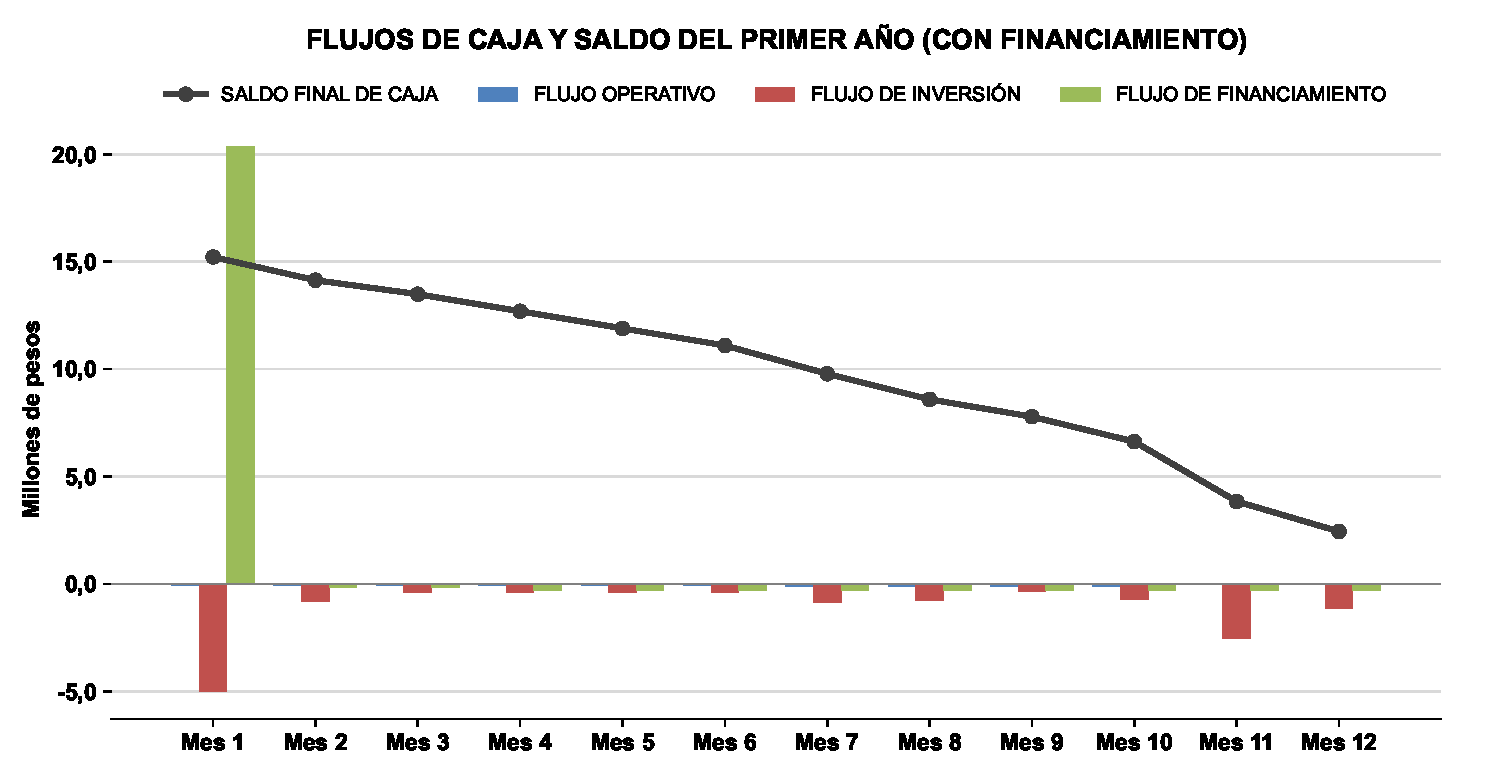
\includegraphics[width=\linewidth]{img/flujo_meses_financiado.pdf}
            \caption{Flujos de caja y saldo del primer año, con financiamiento.}
            \label{fig:flujo_meses_financiado}
        \end{figure}

        \begin{figure}[tbp]
            \centering
            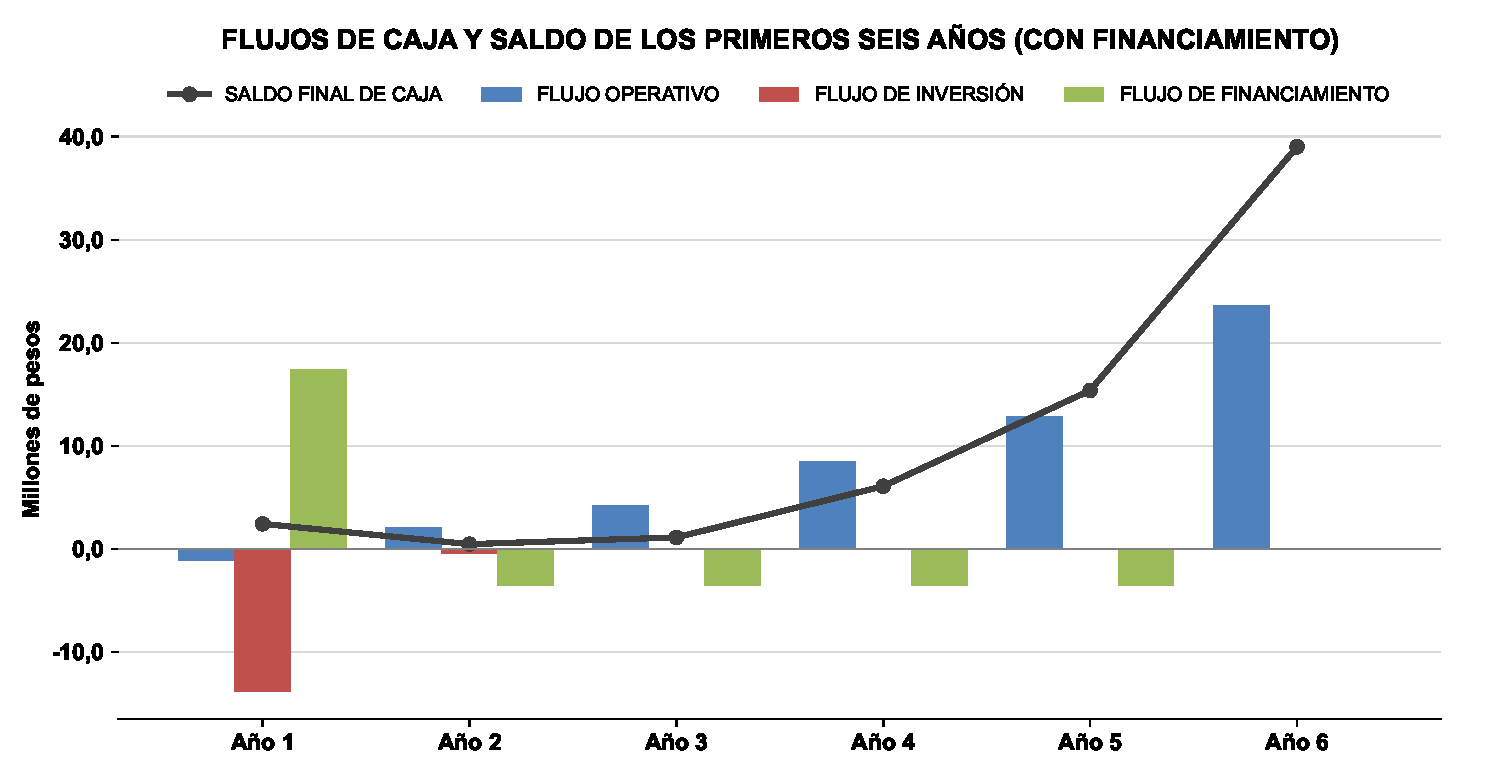
\includegraphics[width=\linewidth]{img/flujo_anios_financiado.pdf}
            \caption{Flujos de caja y saldo de los primeros seis años, con financiamiento.}
            \label{fig:flujo_anios_financiado}
        \end{figure}

        A partir del segundo año la captación crece de manera conservadora: dos suscriptores en el año 2 y tres en el año 3 (clínicas cabecera de Posadas, Oberá y Eldorado), cinco y siete en los años 4 y 5, y doce en el año 6, ya con alcance nacional. La Tabla~\ref{tabla:flujo_anual} resume el flujo de los seis años, y su apertura por rubro se presenta en la Tabla~\ref{tabla:anexo_flujo_anual} del Anexo.

        \begingroup \setstretch{1.1}
        \vspace{0.3cm}\noindent\begin{talltblr}[
            caption = Flujo de caja de los primeros seis años con financiamiento,
            label = tabla:flujo_anual
            ]{
                colspec = {Q[l,m,3.4cm] X[r,m] X[r,m] X[r,m] X[r,m] X[r,m] X[r,m]},
                cells = {font=\scriptsize},
                row{1} = {bg=gray!15, font=\scriptsize\bfseries, halign=c},
                row{4,5,9,10,11} = {bg=gray!15, font=\scriptsize\bfseries},
                hlines, vlines,
                rowsep = 2pt, colsep = 3pt
            }

            Concepto & Año 1 & Año 2 & Año 3 & Año 4 & Año 5 & Año 6 \\

            Ingresos por suscripciones & \$\,360.000 & \$\,4.320.000 & \$\,6.480.000 & \$\,10.800.000 & \$\,15.120.000 & \$\,25.920.000 \\
            Egresos operativos & $-$\$\,1.438.252 & $-$\$\,2.279.452 & $-$\$\,2.279.452 & $-$\$\,2.279.452 & $-$\$\,2.279.452 & $-$\$\,2.279.452 \\
            Flujo de caja operativo & $-$\$\,1.078.252 & \$\,2.040.548 & \$\,4.200.548 & \$\,8.520.548 & \$\,12.840.548 & \$\,23.640.548 \\
            Flujo de caja de inversión & $-$\$\,13.872.740 & $-$\$\,464.000 & \$\,0 & \$\,0 & \$\,0 & \$\,0 \\
            Aporte propio & \$\,8.500.000 & \$\,0 & \$\,0 & \$\,0 & \$\,0 & \$\,0 \\
            Desembolso de los créditos & \$\,12.000.000 & \$\,0 & \$\,0 & \$\,0 & \$\,0 & \$\,0 \\
            Cuotas de los créditos & $-$\$\,3.110.556 & $-$\$\,3.547.408 & $-$\$\,3.547.408 & $-$\$\,3.547.408 & $-$\$\,3.547.408 & \$\,0 \\
            Flujo de caja de financiamiento & \$\,17.389.444 & $-$\$\,3.547.408 & $-$\$\,3.547.408 & $-$\$\,3.547.408 & $-$\$\,3.547.408 & \$\,0 \\
            Flujo de caja neto & \$\,2.438.452 & $-$\$\,1.970.860 & \$\,653.140 & \$\,4.973.140 & \$\,9.293.140 & \$\,23.640.548 \\
            Saldo final de caja & \$\,2.438.452 & \$\,467.591 & \$\,1.120.731 & \$\,6.093.871 & \$\,15.387.010 & \$\,39.027.558 \\

        \end{talltblr}\par\vspace{0.3cm}
        \endgroup

        El momento más exigente es el final del segundo año: los dos suscriptores cubren los costos operativos, pero no las cuotas. Sin aporte propio, la caja acumulada llegaría a $-$\$\,8.032.409 en el mes 24. Por eso el aporte se fija en \$\,8.500.000, de modo que el saldo mínimo resulte positivo (\$\,467.591) y la caja no quede negativa en ningún mes. Desde el tercer año el flujo neto es positivo y el saldo crece hasta \$\,39.027.558 al cierre del sexto año.

        \noindent\colorbox{yellow!10}{%
            \parbox{\dimexpr\linewidth-2\fboxsep}{%
                El flujo original sin financiamiento, previo a estos ajustes, se conserva en las Figuras~\ref{fig:anexo_caja_desarrollo} y~\ref{fig:anexo_caja_años} del Anexo. Las correcciones realizadas sobre aquel modelo se detallan en la hoja Correcciones del archivo de cálculo que acompaña al informe.
            }%
        }
        

    \phantomsection
    \subsection{Precio final del servicio}

        El precio se define a partir de los costos y de la competencia. Los costos fijos anuales de los años 2 a 6 suman \$\,2.279.452 (servidor, herramientas y monotributo). Si además se recupera la inversión pre-operativa en cinco años (\$\,2.774.548 por año), el costo total anual asciende a \$\,5.054.000. Con un promedio de 5,8 suscriptores entre los años 2 y 6, el costo por suscriptor es de unos \$\,72.615 mensuales.

        Sobre esa base, el precio final se fija en \textbf{\$\,180.000 mensuales}, lo que implica un margen de beneficio del 148\,\% sobre el costo unitario. Como los integrantes facturan como monotributistas, el precio no discrimina IVA. Frente a la competencia, equivale a unos 39 informes de Entelai ($\approx$\,\$\,4.586 por informe con IVA), y evita la inversión de USD 20.000 a 40.000 que exige un equipo con \textit{software} propietario. La Tabla~\ref{tabla:precio} resume el cálculo y el punto de equilibrio, calculado según la Ecuación~\ref{eq:pe}:

        \begin{equation}
            Q_e = \frac{CF}{PV - CV_u}
            \label{eq:pe}
        \end{equation}

        \vspace{-0.4 cm}
        \begingroup \setstretch{1.1}
        \vspace{0.3cm}\noindent\begin{talltblr}[
            caption = Determinación del precio final y punto de equilibrio,
            label = tabla:precio
            ]{
                colspec = {X[l,m] Q[r,m,3.6cm]},
                cells = {font=\small},
                row{1} = {bg=gray!15, font=\small\bfseries, halign=c},
                row{6} = {bg=gray!15, font=\small\bfseries},
                hlines, vlines,
                rowsep = 3pt, colsep = 5pt
            }

            Concepto & Valor \\

            Costos fijos anuales, años 2 a 6 ($CF$) & \$\,2.279.452 \\
            Recupero anual de la inversión pre-operativa (5 años) & \$\,2.774.548 \\
            Costo total anual & \$\,5.054.000 \\
            Costo mensual por suscriptor (5,8 suscriptores en promedio) & \$\,72.615 \\
            Precio final de la suscripción mensual & \$\,180.000 \\
            Precio anual por suscriptor ($PV$) & \$\,2.160.000 \\
            Costo variable por suscriptor ($CV_u$) & $\approx$\,\$\,0 \\
            Punto de equilibrio sin las cuotas del crédito & 1,06 $\rightarrow$ 2 suscriptores \\
            Punto de equilibrio con las cuotas del crédito (\$\,5.826.860 anuales) & 2,70 $\rightarrow$ 3 suscriptores \\

        \end{talltblr}\par\vspace{0.3cm}
        \endgroup

        El precio originalmente previsto de \$\,150.000 resultaba insuficiente: con él, la TIR (18,3\,\%) quedaba por debajo de la TREMA una vez incorporados los costos recurrentes de los años 2 a 6 y el monotributo de los integrantes.

    \phantomsection
    \subsection{Tasa de rendimiento mínima aceptable (TREMA)}

        La TREMA es la rentabilidad mínima que exige un inversor para aceptar el proyecto, es decir, su costo de oportunidad (Ecuación~\ref{eq:trema}).

        \begin{equation}
            TREMA = \text{Tasa libre de riesgo} + \text{Prima de riesgo} + \text{Otros}
            \label{eq:trema}
        \end{equation}

        \vspace{-0.4 cm}
        \begingroup \setstretch{1.1}
        \vspace{0.3cm}\noindent\begin{talltblr}[
            caption = Componentes de la TREMA,
            label = tabla:trema
            ]{
                colspec = {Q[l,m,3.6cm] Q[c,m,1.6cm] X[l,m]},
                cells = {font=\small},
                row{1} = {bg=gray!15, font=\small\bfseries, halign=c},
                row{6} = {bg=gray!15, font=\small\bfseries},
                hlines, vlines,
                rowsep = 3pt, colsep = 5pt
            }

            Componente & Valor & Justificación \\

            Tasa libre de riesgo & 4,99\,\% & Rendimiento del bono del Tesoro de EE.UU. a 10 años al 23 de octubre de 2026~\cite{us10y}. \\

            Riesgo país & 7,07\,\% & Índice EMBI de Argentina, 707 puntos básicos al 23 de octubre de 2026~\cite{riesgo_pais}. \\

            Prima de riesgo del proyecto & 10,00\,\% & Emprendimiento sin facturación, que depende de la inscripción ante la ANMAT y de la adopción por parte de los oftalmólogos, en un mercado inicial reducido. \\

            Inflación esperada & No se suma & Los flujos están a precios constantes; sumar la inflación esperada (21,1\,\%~\cite{rem_bcra}) penalizaría dos veces el proyecto. \\

            TREMA & 22,06\,\% & Se redondea a 22,1\,\% en el texto. \\

        \end{talltblr}\par\vspace{0.3cm}
        \endgroup

        Como referencia, la TREMA supera holgadamente el costo de los créditos (15\,\% nominal, negativo en términos reales), por lo que endeudarse para financiar el proyecto es conveniente si este rinde por encima de la TREMA.

    \phantomsection
    \subsection{Valor actual neto (VAN)}

        El VAN descuenta los flujos futuros a la TREMA y les resta la inversión inicial (Ecuación~\ref{eq:van}). Se calcula para el proyecto, sin considerar cómo se financia, y para el inversionista, cuyo flujo incluye el desembolso de los créditos y el pago de las cuotas. La inversión inicial ($I_0$) es la inversión pre-operativa del primer año, de \$\,13.872.740.

        \begin{equation}
            VAN = \sum_{t=1}^{n}\frac{F_{t}}{(1+r)^{t}} - I_{0}
            \label{eq:van}
        \end{equation}

        \vspace{-0.4 cm}
        \begingroup \setstretch{1.1}
        \vspace{0.3cm}\noindent\begin{talltblr}[
            caption = Cálculo del VAN del proyecto y del inversionista (TREMA del 22{,}06\,\%),
            label = tabla:van
            ]{
                colspec = {Q[c,m,1cm] X[r,m] Q[c,m,1.6cm] X[r,m] X[r,m] X[r,m]},
                cells = {font=\small},
                row{1} = {bg=gray!15, font=\small\bfseries, halign=c},
                row{9} = {bg=gray!15, font=\small\bfseries},
                hlines, vlines,
                rowsep = 3pt, colsep = 4pt
            }

            Año ($t$) & Flujo del proyecto & $1/(1+r)^t$ & Flujo descontado & Flujo del inversionista & Flujo descontado \\

            0 & $-$\$\,13.872.740 & 1,0000 & $-$\$\,13.872.740 & $-$\$\,1.872.740 & $-$\$\,1.872.740 \\
            1 & $-$\$\,1.078.252 & 0,8193 & $-$\$\,883.379 & $-$\$\,4.188.808 & $-$\$\,3.431.762 \\
            2 & \$\,1.576.548 & 0,6712 & \$\,1.058.182 & $-$\$\,1.970.860 & $-$\$\,1.322.845 \\
            3 & \$\,4.200.548 & 0,5499 & \$\,2.309.861 & \$\,653.140 & \$\,359.158 \\
            4 & \$\,8.520.548 & 0,4505 & \$\,3.838.611 & \$\,4.973.140 & \$\,2.240.460 \\
            5 & \$\,12.840.548 & 0,3691 & \$\,4.739.327 & \$\,9.293.140 & \$\,3.430.012 \\
            6 & \$\,23.640.548 & 0,3024 & \$\,7.148.540 & \$\,23.640.548 & \$\,7.148.540 \\
            \SetCell[c=3]{r} VAN & & & \$\,4.338.402 & & \$\,6.550.823 \\

        \end{talltblr}\par\vspace{0.3cm}
        \endgroup

        El \textbf{VAN del proyecto es de \$\,4.338.402}. Al ser positivo, los flujos descontados superan la inversión inicial: el proyecto recupera lo invertido, paga la rentabilidad mínima exigida y genera un valor adicional. El VAN del inversionista es mayor (\$\,6.550.823), porque parte de la inversión se financia con deuda a una tasa inferior a la TREMA. Los tres primeros flujos negativos del inversionista ($-$\$\,8.032.409 acumulados) son los que cubre el aporte propio.

    \phantomsection
    \subsection{Tasa interna de retorno (TIR)}

        La TIR es la tasa de descuento que hace que el VAN sea igual a cero (Ecuación~\ref{eq:tir}), y representa la rentabilidad anual propia del proyecto.

        \begin{equation}
            0 = \sum_{t=1}^{n}\frac{F_{t}}{(1+TIR)^{t}} - I_{0}
            \label{eq:tir}
        \end{equation}

        La Tabla~\ref{tabla:indicadores} resume los indicadores. La \textbf{TIR del proyecto es del 29,0\,\%}, superior a la TREMA del 22,1\,\%, y la del inversionista alcanza el 42,8\,\%. Además, la inversión se recupera en 4,05 años sin descontar y en 5,39 años con los flujos descontados, en ambos casos dentro del horizonte de evaluación.

        \begingroup \setstretch{1.1}
        \vspace{0.3cm}\noindent\begin{talltblr}[
            caption = Indicadores de evaluación económica y financiera,
            label = tabla:indicadores
            ]{
                colspec = {X[l,m] Q[r,m,3.2cm] Q[r,m,3.2cm]},
                cells = {font=\small},
                row{1} = {bg=gray!15, font=\small\bfseries, halign=c},
                hlines, vlines,
                rowsep = 3pt, colsep = 5pt
            }

            Indicador & Proyecto & Inversionista \\

            TREMA & 22,1\,\% & 22,1\,\% \\
            Valor actual neto (VAN) & \$\,4.338.402 & \$\,6.550.823 \\
            Tasa interna de retorno (TIR) & 29,0\,\% & 42,8\,\% \\
            Período de recupero simple & 4,05 años & --- \\
            Período de recupero descontado & 5,39 años & --- \\
            Criterio de la guía (TIR $>$ TREMA y VAN $>$ 0) & Se cumple & Se cumple \\

        \end{talltblr}\par\vspace{0.3cm}
        \endgroup

    \phantomsection
    \subsection{Análisis de sensibilidad}

        La Tabla~\ref{tabla:sensibilidad} muestra cómo varían los indicadores al modificar un parámetro por vez. La última columna indica el aporte que haría falta en cada escenario para que la caja no quede negativa.

        \begingroup \setstretch{1.1}
        \vspace{0.3cm}\noindent\begin{talltblr}[
            caption = Análisis de sensibilidad del proyecto,
            label = tabla:sensibilidad
            ]{
                colspec = {X[l,m] Q[r,m,2.3cm] Q[c,m,1.4cm] Q[r,m,2.3cm] Q[c,m,1.5cm] Q[r,m,2.3cm]},
                cells = {font=\footnotesize},
                row{1} = {bg=gray!15, font=\footnotesize\bfseries, halign=c},
                row{2} = {bg=gray!15},
                hlines, vlines,
                rowsep = 3pt, colsep = 4pt
            }

            Escenario & VAN del proyecto & TIR del proyecto & VAN del inversionista & TIR del inversionista & Mínimo de caja sin aporte \\

            Caso base & \$\,4.338.402 & 29,0\,\% & \$\,6.550.823 & 42,8\,\% & $-$\$\,8.032.409 \\
            Precio de \$\,150.000 ($-$17\,\%) & \$\,164.761 & 22,3\,\% & \$\,2.377.182 & 30,0\,\% & $-$\$\,9.239.269 \\
            Precio de \$\,210.000 (+17\,\%) & \$\,8.512.043 & 34,9\,\% & \$\,10.724.464 & 54,4\,\% & $-$\$\,7.252.409 \\
            Un suscriptor menos por año & $-$\$\,722.661 & 20,9\,\% & \$\,1.489.760 & 26,6\,\% & $-$\$\,11.699.269 \\
            Costos +20\,\% & \$\,197.713 & 22,3\,\% & \$\,2.410.134 & 27,8\,\% & $-$\$\,11.643.298 \\
            Lanzamiento demorado 6 meses & $-$\$\,1.161.805 & 20,1\,\% & \$\,1.050.616 & 25,5\,\% & $-$\$\,10.945.839 \\
            Un solo crédito de \$\,6.000.000 & \$\,4.338.402 & 29,0\,\% & \$\,5.444.612 & 33,4\,\% & $-$\$\,10.725.664 \\
            TREMA del 17,1\,\% (prima del 5\,\%) & \$\,8.542.416 & 29,0\,\% & \$\,9.581.851 & 42,8\,\% & $-$\$\,8.032.409 \\
            TREMA del 27,1\,\% (prima del 15\,\%) & \$\,1.067.755 & 29,0\,\% & \$\,4.260.731 & 42,8\,\% & $-$\$\,8.032.409 \\
            Consultoría oftalmológica completa (sin convenio) & \$\,1.758.402 & 24,6\,\% & \$\,3.970.823 & 31,8\,\% & $-$\$\,10.612.409 \\

        \end{talltblr}\par\vspace{0.3cm}
        \endgroup

        Los parámetros más sensibles son la demanda y los plazos. Con un suscriptor menos por año o con un lanzamiento demorado seis meses, el VAN del proyecto se vuelve negativo, aunque el del inversionista se mantiene positivo gracias al apalancamiento. Bajar el precio a \$\,150.000 o aumentar los costos un 20\,\% deja al proyecto en el límite de la TREMA. Si se aprobara un solo crédito, la rentabilidad seguiría siendo aceptable, pero el aporte propio necesario subiría a unos \$\,11.000.000.

    \phantomsection
    \subsection{¿Es atractivo para el inversionista?}

        Sí, aunque con condiciones. KERALYTIX resulta rentable para el inversionista dando un TIR del proyecto (29,0\,\%) supera la TREMA (22,1\,\%) y el VAN es positivo (\$\,4.338.402). El atractivo se apoya además en:

        \begin{itemize}
            \item \textbf{Apalancamiento favorable:} los créditos cuestan un 15\,\% fijo, por debajo de la TREMA y negativo en términos reales, lo que eleva la TIR del inversionista al 42,8\,\%.

            \item \textbf{Escalabilidad:} el costo de atender a un suscriptor adicional es prácticamente nulo, por lo que el flujo crece casi en la misma proporción que las suscripciones.

            \item \textbf{Ventaja competitiva:} no hay competidores nacionales con un producto específico para queratocono, y la inscripción ante la ANMAT constituye una barrera de entrada para nuevos competidores.

            \item \textbf{Beneficio para el sistema de salud:} una detección temprana puede evitar tratamientos que cuestan entre veinte y más de sesenta veces lo que un estudio topográfico (ver Impacto económico).
        \end{itemize}

        Sin embargo, el margen sobre la TREMA es moderado y depende del ritmo de captación: una demora de seis meses o un suscriptor menos por año vuelven negativo el VAN del proyecto. Por eso KERALYTIX resulta atractivo para un inversor que acepte el riesgo de una etapa temprana, siempre que se cumplan las condiciones de financiamiento que se detallan a continuación.

    \phantomsection
    \subsection{Consideraciones sobre el esquema de financiamiento}

        La viabilidad calculada depende de las siguientes condiciones, que deben confirmarse con un oficial de crédito del FCM antes de iniciar el trámite:

        \begin{itemize}
            \item \textbf{Dos créditos para un mismo proyecto:} el tope de \$\,6.000.000 es por solicitante, y cada pedido requiere su propio formulario, presupuestos, localización y habilitación. El FCM podría considerar ambos pedidos como un único emprendimiento y aprobar solo uno (R9).

            \item \textbf{Tasa sujeta a la TAMAR:} la tasa es el 60\,\% de la TAMAR vigente al firmar el contrato. Si la TAMAR sube antes de la firma, la cuota aumenta.

            \item \textbf{Gastos de otorgamiento:} los costos de escribanía, seguros, tasación (si hay hipoteca) e inscripción de la prenda no están incluidos en el flujo.

            \item \textbf{Destino de los fondos:} los honorarios solo son financiables si el FCM los acepta como investigación y desarrollo, y la porción de capital de trabajo debe devolverse en doce meses (R11). Si no se aceptan, el crédito se reduce a los rubros admitidos y la diferencia se cubre con aporte propio.

            \item \textbf{Garantes y bienes de terceros:} cada crédito necesita su garantía. Un garante debe acreditar ingresos de al menos 5 veces la cuota, y un vehículo o inmueble familiar queda comprometido hasta cancelar el crédito.

            \item \textbf{Monotributo e Ingresos Brutos:} cada integrante debe inscribirse antes de firmar. Con 12 suscriptores, los ingresos del año 6 (\$\,12.960.000 por integrante) superan el tope anual de la categoría A (\$\,12.009.410~\cite{monotributo_2026}), por lo que será necesario recategorizarse o constituir una sociedad.

            \item \textbf{Localización:} se debe acreditar el lugar del emprendimiento, por ejemplo, mediante un comodato con la UNaM o con una incubadora del Parque Tecnológico Misiones.

            \item \textbf{Aporte propio:} los \$\,8.500.000 superan ampliamente el capital inicial de los integrantes, por lo que dependen de ahorros y aportes familiares. Es la condición principal para que la caja no quede negativa en el segundo año.

            \item \textbf{Fuentes de la información:} las condiciones del FCM se tomaron de sus preguntas frecuentes, infografías y notas de prensa de 2026, y pueden modificarse.
        \end{itemize}
